\documentclass{article}
\usepackage{graphicx}
\usepackage{xcolor}
\usepackage{subcaption}
\usepackage[margin=1.0in]{geometry}
\usepackage{float}
\usepackage{ulem}
\usepackage{amsmath}
\usepackage{mathtools}
\usepackage{wrapfig}
\begin{document}
\begin{abstract}
Constructing model Hamiltonians which can accurately describe the energies and properties of the lowest lying eigenstates for strongly correlated electron systems is a pressing problem in modern condensed matter physics.
In this paper we systematically develop a many-body model for the neutral CuO molecule using a generalizable \textit{ab-initio} Quantum Monte Carlo (QMC) density matrix downfolding (DMD) method and discuss details of the fitting procedure.
Exact solutions to our final regressed model accurately reproduce properties and energies of the lowest lying eigenstates of the CuO molecule.
Our results indicate that the DMD procedure can serve as a systematic method for developing many-body effective theories for strongly correlated electron systems.
\end{abstract}

\section{Introduction}
Systematically developing model Hamiltonians which can accurately describe the energies and properties of the lowest lying eigenstates for strongly correlated electron systems is a pressing problem in modern condensed matter physics. 
Examples of such materials are high-temperature superconductors and other transition metal oxides.
Low-energy excitations of these systems typically involve collective spin, lattice, and charge degrees of freedom with intermediate couplings.
Consequently, many of these systems have competing exotic long range ordering, for example the hypothesized competition between antiferromagnetic order and d-wave superconducting order in the cuprates.
The main difficulty in describing these materials is that they do not exhibit behavior which can be described by an effective single particle theory nor perturbatively in either weak or strong coupling limits.

The necessity for non-perturbative, many-body models in describing the low-lying excited states of strongly correlated electron systems poses a difficult challenge when developing model Hamiltonians for real world systems.
Fermi liquid theory is the prototypical example of a one-body non-perturbative effective theory for metals.
The low-energy effective theory has long-lived non-interacting single particle excitations near the Fermi surface and the Coulomb interaction is treated non-perturbatively.
The anti-ferromagnetic Heisenberg model is a good example of a many-body perturbative effective theory for Mott insulators.
The low-energy effective theory is built of many-body spin excitations which are derived from perturbing from a strong coupling limit.
These types of models fail when used to model many strongly correlated electron systems, and consequently various non-perturbative many-body models like the t-J, 3-band Hubbard, and Kanamori models have emerged as candidates.
While these models are computational tractable to solve, it is unclear whether they can describe the complexity of real systems, or how one would go about developing a more suitable model for a given material.

Common approaches to building suitable model Hamiltonians for strongly correlated materials involve using single particle theories like density functional theory (DFT).
One-body terms are typically obtained by projecting the solutions from the DFT band structure onto a localized single-particle basis, giving an estimate of hoppings and occupations on a lattice model.
Two-body terms in the model are developed by assuming a screened Coulomb interaction based on constrained DFT or RPA.
Aside from this method, Lowdin methods coupled to a stochastic method and canonical transformations have also been used to develop effective theories.
These methods have the draw back that the constructed effective theory typically does not come with any estimate of the quality of the model, therefore making model validation a phenomenological task which can lead to unclear biases in the model construction.

In this paper we systematically fit a many-body model
which can accurately describe energies and properties of low-lying eigenstates for the neutral CuO molecule using a generalizable \textit{ab-initio} QMC DMD method as a stepping stone towards application to bulk strongly correlated materials.
The neutral CuO molecule has been a subject of intense theoretical and experimental study due to the complex structure of its low-energy space.
While the low-energy excitations in the doublet sector of the CuO molecule are well understood, singlet selection rules for spectroscopic measurements and the doublet ground state leave the quartet sector of excitations unexplored.
The CuO molecule is hence a good playground for testing and developing the DMD method as there are some well understood excitations which our model should describe accurately and a set of poorly understood excitations which our model can give some insight into.
The relative simplicity of the system allows us to rigorously detail each step of the DMD procedure, particularly sampling and regression techniques as well as quantifiable model validation.

\section{Methods}
\subsection{Density Matrix Downfolding (DMD)}
The DMD procedure allows us to develop low-energy effective theories for physical systems in a systematic manner beginning with the \textit{ab-initio} Hamiltonian:
\begin{equation}
\hat{H}_\text{ab} = -\frac{1}{2} \sum_{i} \nabla_i^2 - \sum_{i,I}\frac{Z}{|r_i - R_I|} + \sum_{i<j}\frac{1}{|r_i - r_j|}
\label{eq:Hab}
\end{equation}
where $i$ indicates electrons and $I$ nuclei, and the unit of energy is Hartree (Ha).
In this paper we will be working under the Born-Oppenheimer approximation and core electrons will be treated using pseudo-potentials.
The procedure defines a method for downfolding the \textit{ab-initio} energy functional and Hilbert space onto an effective energy functional defined on a low-energy subspace of the Hilbert space 
\begin{equation}
(E_\text{ab}, \mathcal{H}) \xrightarrow{\text{DMD}} (E_\text{eff}, \mathcal{LE} \subset \mathcal{H}), \text{ s.t. }
\forall |\Psi\rangle \in \mathcal{LE}, \ E_\text{eff}[\Psi] - E_\text{ab}[\Psi] = \epsilon[\Psi] + E_0.
\label{eq:DMD}
\end{equation} 
The energy functionals can be written as expectations over Hamiltonian operators $E_\text{ab} = \langle \Psi | \hat{H}_\text{ab} |\Psi \rangle$, $E_\text{eff} = \langle \Psi | \hat{H}_\text{eff} |\Psi \rangle$, $\epsilon$ represents the error in our effective theory, and $E_0$ is a constant energy shift.
Broadly the DMD method consists of four steps which will be discussed in detail later: 
A) Defining the space of low-energy excitations which $E_\text{eff}$ should be able to describe accurately.
B) Sampling, at minimum, a set of states in $\mathcal{H}$ which probe the chosen low-energy excitations in a statistically independent manner. The selected states need not be eigenstates. 
C) Constructing a set of candidate models which are linear in reduced density matrix (RDM) descriptors with variable coefficients $\{c\}$
\begin{equation}
E_\text{eff} = \sum_k c_k \langle \Psi | \hat{d}_k |\Psi \rangle + E_0.
\label{eq:Eeff}
\end{equation}
Here $\hat{d}_k$ are Hermitian operators typically composed of 1- or 2-RDM elements. 
Examples of possible $\hat{d}_k$ are number operators $\hat{n}_i$ and exchange operators $\vec{S}_i \cdot \vec{S}_j$.
Additionally, a single particle basis must be built to express RDM elements on and should be chosen such that variations among states in $\mathcal{LE}$ are mostly described by variations in the projection of these states onto the basis.
D) Using the samples to fit the coefficients $\{c\}$ by linear regression such that $E_\text{eff}$ satisfies the conditions in \eqref{eq:DMD} with the smallest error $\epsilon$ possible. 
The fitting procedure is typically an ordinary linear regression, however, one may use a custom cost function in the regression as well. 
In order to conduct the linear regression for a functional like \eqref{eq:Eeff}, one needs to calculate for each state sampled from $\mathcal{LE}$ the expectation values of $\hat{H}_\text{ab}$ and every descriptor $\{\hat{d}_k\}$ used in the regression.
In principle, if conducted with no approximations, the DMD method is rigorously guaranteed to obtain exact results, namely $\epsilon[\Psi] = 0$.

\subsection{Fixed-node diffusion Monte Carlo (FN-DMC)}
When downfolding $\hat{H}_\text{ab}$ we will use FN-DMC to access states in $\mathcal{LE}$ and accurately calculate their \textit{ab-initio} energies and RDM elements.
Diffusion Monte Carlo (DMC) is a quantum Monte Carlo method which projects out the ground state of a Hamiltonian given some initial trial wave function.
Consider a trial wave function $|\Psi_T\rangle$ and the Hamiltonian $\hat{H}_\text{ab}$ with ground state $|\Phi_0\rangle$. We apply the projector $e^{-\tau \hat{H}_\text{ab}}$ as $\tau \rightarrow \infty$ to $|\Psi_T \rangle$
\begin{equation}
\lim_{\tau \rightarrow \infty} e^{-\tau \hat{H}_\text{ab}} |\Psi_T\rangle 
\equiv \lim_{\tau \rightarrow \infty} |\Psi_\text{DMC}(\tau)\rangle \propto \langle \Phi_0|\Psi_T\rangle |\Phi_0\rangle,
\end{equation}
projecting out the ground state as long as the trial wave function we choose is not orthogonal to the ground state. 
The stochastic implementation involves moving samples from the trial function $\Psi_T(R)$ using the Green function $G(R, R^\prime, \tau) = \langle R | e^{-\tau(\hat{H}_\text{ab} - E_T)} | R^\prime \rangle$. Since $H_\text{ab} = T + V$, kinetic and potential energy terms, the Green function is approximated by a Trotter expansion $G(R, R^\prime, \tau) = \langle R | e^{-\tau(\hat{H} - E_T)} | R^\prime \rangle \sim \Big[e^{-d\tau(V(R) + V(R^\prime))/2} \langle R| e^{-d\tau(\hat{T} - E_T)}|R^\prime \rangle + O(d\tau^2) \Big]^N $ where $d\tau = \tau/N$.
This expansion can be interpreted as an interative procedure where samples are moved N times with a small timestep $d\tau$ until convergence.
The constant $E_T$ is a trial energy used to control the normalization of $\Psi_\text{DMC}(\tau, R)$ and is updated at each move.
This implementation, however, suffers from a fermion sign problem. 
We deal with this sign problem through a fixed-node approximation, where the nodal surface of $\Psi_\text{DMC}(\tau, R)$ is forced to match that of the initial trial wave function for all $\tau$.
This approximation makes FN-DMC variational, and will only return the exact ground state of $\hat{H}_\text{ab}$ if the nodal surfaces of $|\Psi_T\rangle$ and $|\Phi_0\rangle$ are identical.
We make use of this variational principle to access low-energy states within $\mathcal{H}$ by choosing trial wave functions with nodes that differ from the nodes of $|\Phi_0 \rangle$.
To calculate the expectation value of an operator $\hat{A}$ in FN-DMC we will use a mixed estimator $\langle \Psi_{DMC}(\tau) |\hat{A} | \Psi_T \rangle/\langle \Psi_\text{DMC}(\tau) | \Psi_T \rangle$ which allows us to use the importance sampled distribution $f = \Psi_\text{DMC}(\tau)\Psi_T$ for our Monte Carlo estimates.
Details for calculating reduced density matrix elements in FN-DMC can be found in Wagner.

\subsection{Defining $\mathcal{LE}$ for CuO molecule}
We construct our $\mathcal{LE}$ based on recent anion photoelectron spectroscopy (APES) measurements of the low-lying excited states of the nuetral CuO molecule. 
The lowest energy excitations measured, which lie below 2eV, involve primarily the O 2p$_z$, 2p$_\pi$ and Cu 4s orbitals, which are fully-filled, half-filled and empty in the ground state respectively.
Beginning at 2.2 eV are excitations which remove a single electron from the fully filled Cu 3d shell and add them to either the O 2p$_\pi$ or Cu 4s orbitals.
The neutral copper atom also carries a Hund's coupling between the d and s orbitals of about $\sim$ 0.5 eV, the effects of which would be measurable among the states in $\mathcal{LE}$ as long as states of both doublet and quartet states are included.
In order to probe all of these low-energy excitations we select a low-energy space
\begin{equation}
\mathcal{LE} = \text{Span(}\{ |\Psi \rangle | \langle \Psi | \hat{n}_{3d} | \Psi \rangle \ge 9,\ \hat{H}_\text{ab}|\Psi\rangle = E |\Psi\rangle \}\text{)}.
\label{eq:LE}
\end{equation}
Our particular focus will be on describing most accurately the properties and energies of eigenstates up to $\sim$2eV, as measurements on higher energy states observe a nearly continuous block of states which include vibrational modes.

\subsection{Sampling $\mathcal{LE}$}
Our sample space was generated by using multi-Slater-Jastrow trial wavefunctions in FN-DMC. 
In principle we could probe every low-energy excitation in $\mathcal{LE}$ in a statistically independent manner by just sampling the eigenstates within $\mathcal{LE}$ and including various non-eigenstates within $\mathcal{LE}$ as well to ensure robust statistics.
In practice we do not have access to these eigenstates and approximate methods are required to sample the low-energy space. 
Consider a trial wavefunction of the form $e^{J_i} |\text{D}_i\rangle$, where $e^{J_i}$ is a three-body Jastrow factor and $|\text{D}_i\rangle$ is a determinant of some single particle orbitals.
If the nodes of $|\text{D}_i\rangle$ are similar to the nodes of an eigenstate $|\Phi_i\rangle \in \mathcal{LE}$, then the properties and energy calculated from FN-DMC using this trial wavefunction will approximate those of the eigenstate, with the degree of approximation depending on the quality of the trial function nodal structure.
If we were able to find for each $|\Phi_i \rangle \in \mathcal{LE}$ such a $|\text{D}_i\rangle$ then we can approximate any state in $\mathcal{LE}$ as
\begin{equation}
|\Psi\rangle = \sum_i c_i |\Phi_i\rangle \sim \sum_i c_i \lim_{\tau \rightarrow \infty} e^{-\tau \hat{H}_\text{ab}} (e^{J_i} |D_i\rangle) \xrightarrow{J_i = J} \lim_{\tau \rightarrow \infty} e^{-\tau \hat{H}_\text{ab}} (e^{J}\sum_{i} c_i|\text{D}_i\rangle).
\label{eq:sampling}
\end{equation}
The last equality is valid if $\forall i\  J_i = J$, allowing us to map $|\Psi \rangle \in \mathcal{LE}$ to the end result of an FN-DMC calculation using a multi-Slater-Jastrow trial wavefunction. We use symmetry-targeted unrestricted Kohn-Sham (UKS) to generate our determinants $|\text{D}_i\rangle$ using a B3LYP functional, which has been shown to accurately reproduce ground state nodal properties of transition-metal oxide molecules, a Trail-Needs pseudopotential, and the VTZ Trail-Needs basis using the package PySCF.
The symmetry-targeted UKS method allows us to fix the total spin projection S$_z$ and the total number of electrons in a particular irreducible representation (irrep) of the symmetry group under use, $\text{A},\ \text{E}_\text{1x},\ \text{E}_\text{2y}$ etc.
This method allows us to access almost every excitation in $\mathcal{LE}$, however, there are some cases of two or more low-energy states within $\mathcal{LE}$ which have identical S$_z$ and number of electrons per irrep.
An example of this dilemma would be the ground state and the state with an excitation from Cu 3d$_{xz} \rightarrow $  O 2p$_x$.
In these few cases the higher energy excited $|\text{D}_i\rangle$ is inaccessible and the corresponding $|\Phi_i\rangle$ is excluded from the sum in \eqref{eq:sampling}, restricting our sample space to a subspace of $\mathcal{LE}$.
Methods like constrained DFT also failed to converge the inaccessible $|\text{D}_i\rangle$.
We will discuss the consequences of this restriction later on.
A single three-body Jastrow factor $J$ was used for every $|\text{D}_i\rangle$ and was optimized on the lowest energy UKS state using a linear energy optimization method.
The FN-DMC calculations were conducted with T-moves, to make the calculation variational while using pseudopotentials, with a timestep of $\tau = 0.01$.
The coefficients $\{c_j\}$ for our sample states were chosen via a shell-sampling method. 
We begin by fixing the coefficient $c_0 = \sqrt{w}$ where $w \in \{1.0, 0.8, ..., 0.2\}$. 
For each choice of $w$ we sample n = 5 states by randomly selecting the unassigned coefficients from a uniform distribution such that $\sum_i c_i^2 = 1$. 
This procedure generates shells of samples at decreasing distance from the eigenstate $|\Phi_0\rangle$. 
We can then loop over all $i$ to generate shells near each eigenstate.
This sampling scheme tends to be sparse where the density of states of $\hat{H}_\text{ab}$ is low and therefore extra samples are generated in regions of sparse sample density \textit{post-hoc}. 

\subsection{Constructing candidate models}
Parameterizing our effective model requires constructing a basis on which to calculate our \textit{ab-initio} 1-/2-RDM elements and selecting a set of descriptors from which we would like to build our model.
As discussed, the lowest energy excitations in the CuO molecule are between the Cu 3d, 4s and O 2p orbitals, meaning that our basis needs to span these orbitals. 
We constructed two such bases: a localized intrinsic atomic orbital (IAO) basis and a molecular orbital (MO) basis.
The IAO basis was built on all Cu 3d, 4s and O 2p molecular orbitals from the $|\text{D}_i\rangle$ used to construct our sample states.
The MO basis consists of the Cu 3d, 4s and O 2p molecular orbitals from the lowest energy restricted open-shell Kohn-Sham (ROKS) solution with $x \leftrightarrow y$ spatial symmetry, a O 2p$_z \rightarrow$ O 2p$_\pi$ excitation.
As these two bases are used to describe the same space, they are related by an orthogonal transformation which will allow us to map between them if necessary.
This choice for the MO basis ensures that our basis elements are spin-independent and respect the spatial symmetries of the molecule.
In order to describe the low-energy degrees of freedom in the CuO molecule our model will require occupation energies and hybridizations between the Cu 3d, 4s and O 2p atomic orbitals.
A sparser representation can be found using a MO basis, since occupation operators in the MO basis contain information on both occupation and hybridization in an atomic basis. 
The lack of doubly occupied Cu 4s states in the low-energy spectrum of CuO indicate the necessity of a Hubbard U term on the Cu 4s.
This is corroborated by the fact that the FN-DMC energy of the lowest-lying sampled state with a doubly occupied Cu 4s orbital is 7 eV above the lowest energy sampled state.
Further, we include a Hund's coupling between the Cu 4s and Cu 3d orbitals in our model based on the existence of a similar Hund's coupling 
for the copper atom.
These two interaction terms are best represented in the IAO basis as they are intuitively interactions between localized orbitals.
In addition to these important parameters, we will consider models which contain any number of hybridizations between the MOs to account for orbital relaxation between excited states in the CuO molecule.
In total our space of canditate models is then 
\begin{equation}
\begin{split}
\{\bar{n}_{4s}, \bar{n}_{p_\pi}, \bar{n}_{p_z}, \hat{n}_{4s\uparrow} \hat{n}_{4s\downarrow},\sum_{i \in \{xy, xz, ...\}}\vec{S}_{4s}\cdot \vec{S}_{d_i}\} \ + \\
\text{P}(\bar{c}_{d_\pi}^\dagger \bar{c}_{p_\pi} + h.c.,\ \bar{c}_{d_z^2}^\dagger \bar{c}_{p_z} + h.c.,\ \bar{c}_{4s}^\dagger \bar{c}_{p_z} + h.c.,\ \bar{c}_{d_z^2}^\dagger \bar{c}_{4s} + h.c.)
\end{split}
\label{eq:models}
\end{equation}
where P denotes the power set and operators are defined on the IAO basis unless denoted by a bar, in which case the operator is built on the MO basis. The coefficients for each term above will be denoted $\bar{\epsilon}_{4s},\ \bar{\epsilon}_{p_\pi},\ \bar{\epsilon}_{p_z},\ U_s,\ J_{sd},\ \bar{t}_\pi,\ \bar{t}_{dz},\ \bar{t}_{sz},\ \bar{t}_{ds}$. The operator $\bar{n}_{3d}$ is not included in any models as it is linearly dependent on all other occupation energies through the relationship $\bar{n}_{3d} + \bar{n}_{p_z} + \bar{n}_{p_\pi} + \bar{n}_{4s} = N_\text{elec} = \text{15}$. The symbol $\pi$ denotes a contraction over $x, y$ for p orbitals and $xz,\ yz$ for d orbitals. The symbol $\delta$, introduced later, denotes a contraction over $xy,\ x^2-y^2$ for d orbitals.

\pagebreak
\subsection{Fitting candidate models}
After fitting each of the potential models in \eqref{eq:models} using ordinary linear regression (OLS) and solving the resultant models using exact diagonalization, we find a set of models which describe the energy functional on our sample set accurately but whose eigenstates and spectra differ as a consequence of intruder states below an energy of 2eV. 
The sixteen different models all regress with R$^2 >$ 0.95 on our sample data, however some models are more robust than others. 
Models which have coefficients that are zero within 95\% confidence intervals, computed through bootstrap estimates, are removed from consideration.
We then take the left over models, rotate every operator and coefficient into the IAO basis through an appropriate orthogonal transformation, and exactly diagonalize the models.
Any models which have an average errorbar in eigenvalues, also estimated by bootstrapping, greater than 0.25 eV are ignored.
Each of the remaining six models describe our sample set accurately, have robust non-zero coefficients, and have small error bars in eigenvalues.
However, the eigenstates below 2eV differ greatly between these models as illustrated in Figure \ref{fig:InitED}.

\begin{figure}[H]
\centering
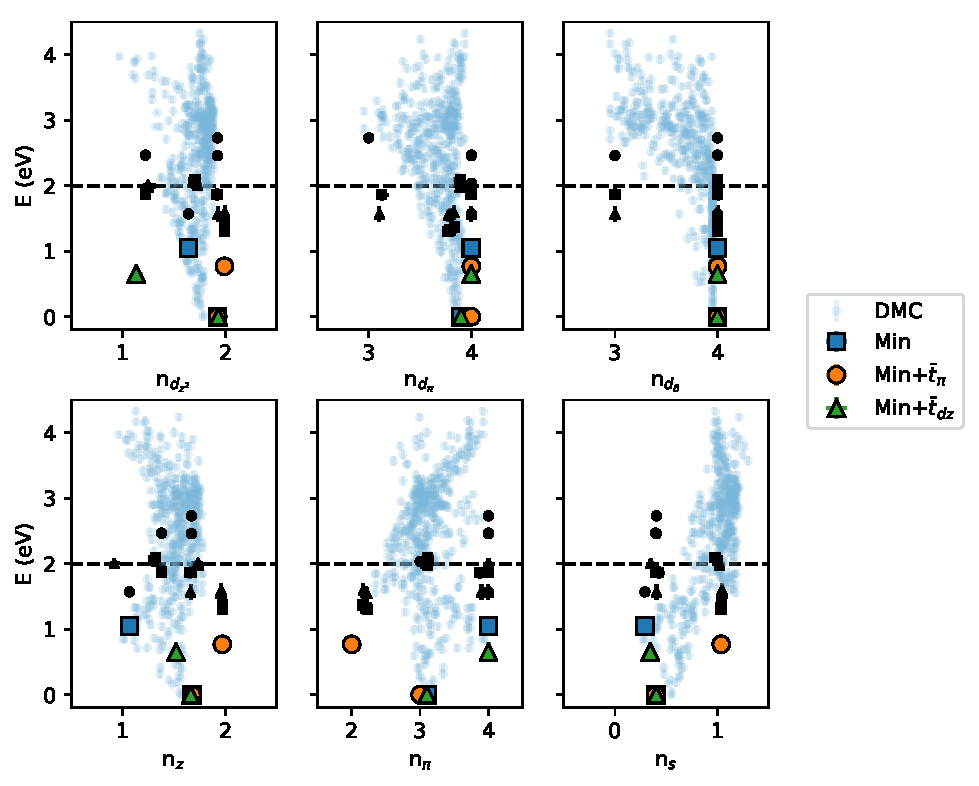
\includegraphics[width=0.7\linewidth]{../qwalk/old/ub3lyp_s1_/analysis/figs/init_ed.pdf}
\caption{Results of exact diagonalization showing the energies and properties of the first twenty eigenstates for three candidate models fit using ordinary linear regression. The ground state and first excited state are colored and have enlarged markers for clarity. Error bars are 95\% CI calculated by a bootstrap estimate.}
\label{fig:InitED}
\end{figure}

All three models have a first excited state around 1eV, but only in the minimal model does this state fall near the sample set used for the fitting, and is the only model in which this state corresponds to the correct excitation O 2$p_z \rightarrow $ O 2p$_\pi$ as seen in experiment.
In contrast, the first excited state for the other two models are visibly distant from our sample set and do not correspond to the experimental first excited state.
The large distance of these eigenstates from our sample set indicates that their predicted eigenvalues may suffer from large extrapolation errors, and as such we will call them \textit{intruder} states.
In Figure \ref{fig:Intruder} we present all eigenstates among the six potential models which we classify as intruders.
While using a Mahalanobis distance is a typical strategy for outlier (intruder) detection, it is only useful for distributions which are approximately normal.
Our sample space does not resemble a (multivariate) normal distribution in any way, so we instead look at the average distance of the five nearest neighbor samples to an eigenstate.
If the average distance is larger than 0.9, which in this case happens to divide eigenstates into intruders above and not below cleanly, it is classified as an intruder state.
In the situation that multiple models share an intruder state, only the intruder state with the farthest average distance is included.

\begin{figure}[H]
\centering
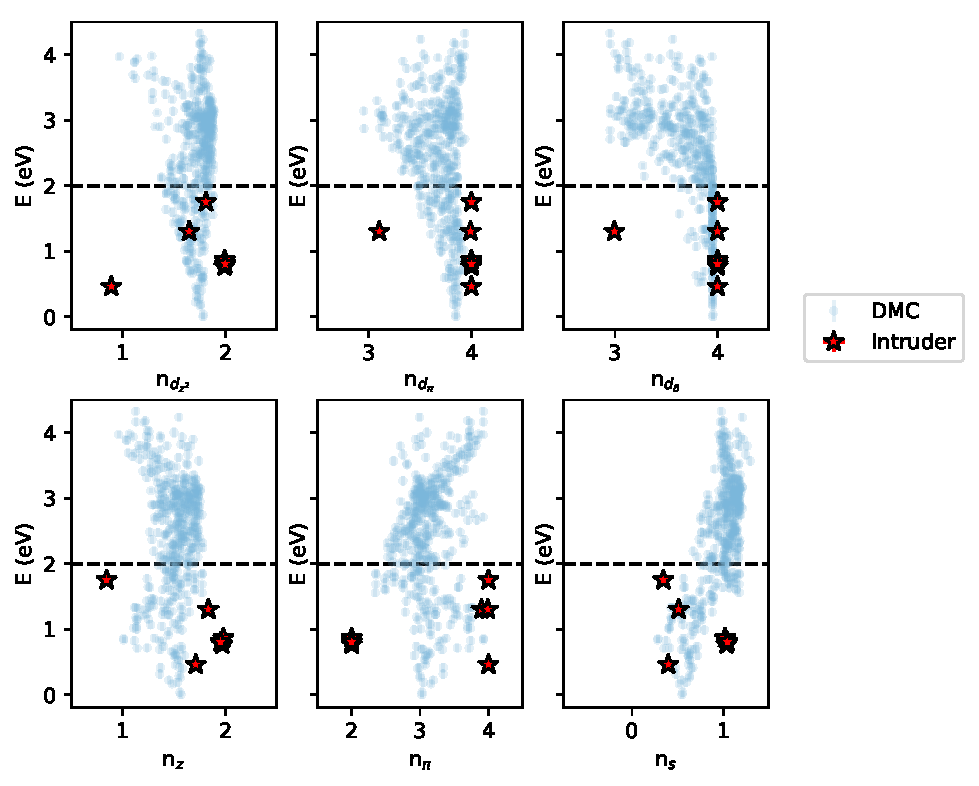
\includegraphics[width=0.7\linewidth]{../qwalk/old/ub3lyp_s1_/analysis/figs/intruder.pdf}
\caption{Collection of unique intruder states from our six potential models selected using a k-nearest neighbor approach with k = 5.}
\label{fig:Intruder}
\end{figure}

Given that our intruder states correspond to states within $\mathcal{LE}$ but outside our sample set, they must live within the span of the eigenstates which were excluded in our sampling scheme as described before.
This is evidenced by the fact that two of the intruder states correspond explicitly to excitations we could not access: Cu 3d$_{z^2} \rightarrow $ O 2p$_\pi$ and  Cu 3d$_\pi \rightarrow $ O 2p$_\pi$.
In fact, these are the only two singly excited states which we could not access with our sampling scheme.
While inaccessible, we can approximate these states by single rigid MO excitations above the UKS ground state, which results in states with a FN-DMC energy above 4eV.
Including a generous 2eV reduction in FN-DMC energy due to orbital relaxation, we estimate that these two states should lie at least 2eV in energy. 
Since all the other inaccessible eigenstates are double or higher order excitations, our very approximate exploration of the inaccessible parts of $\mathcal{LE}$ leaves us with a reasonable prior: intruder states should lie above 2eV in energy in our effective theories.
We can enforce this prior by adding a term to our ordinary linear regression cost function
\begin{equation}
\text{Cost} = \sum_{i} (E_\text{eff}[\Psi_i] - E_\text{ab}[\Psi_i])^2 + \lambda \sum_{p}\text{QHL}(2 - E_\text{eff}[\Psi_p]),\ \text{QHL}(x) = \Theta(x)x^2
\label{eq:cost}
\end{equation}
where $\lambda>0$ is a parameter which can be varied, QHL is a quadratic hinge loss, $\Theta$ is the Heaviside step function, the index $i$ is over our sampled states and $p$ over the selected intruder states.
Increasing the value of $\lambda$ leads to a stronger penalty for models which do not satisfy our prior.

\section{Results and Discussion}
\subsection{Regression with a prior}
Using our new cost function we find a set of models which accurately describe our sample data, have very similar spectra and eigenvectors, and do not contain intruder states below the 2eV prior. 
Shown in Figure \ref{fig:Prior} show the R$^2$ score and QHL for different models fit at $\lambda \in [0,20]$. 
The R$^2$ score stays above 0.95 for all models and $\lambda$, and the QHL converges quickly to nearly zero at $\lambda = 20$ for all six models. 
We conclude that all six models at $\lambda = 20$ should be considered good models as they satisfy our prior and also explain our sample set accurately. 
Also shown are $E_\text{eff}, E_\text{ab}$ for our samples using the minimal model at $\lambda = 20$ to illustrate the high fit quality even with a large $\lambda$.

\begin{figure}[H]
\centering
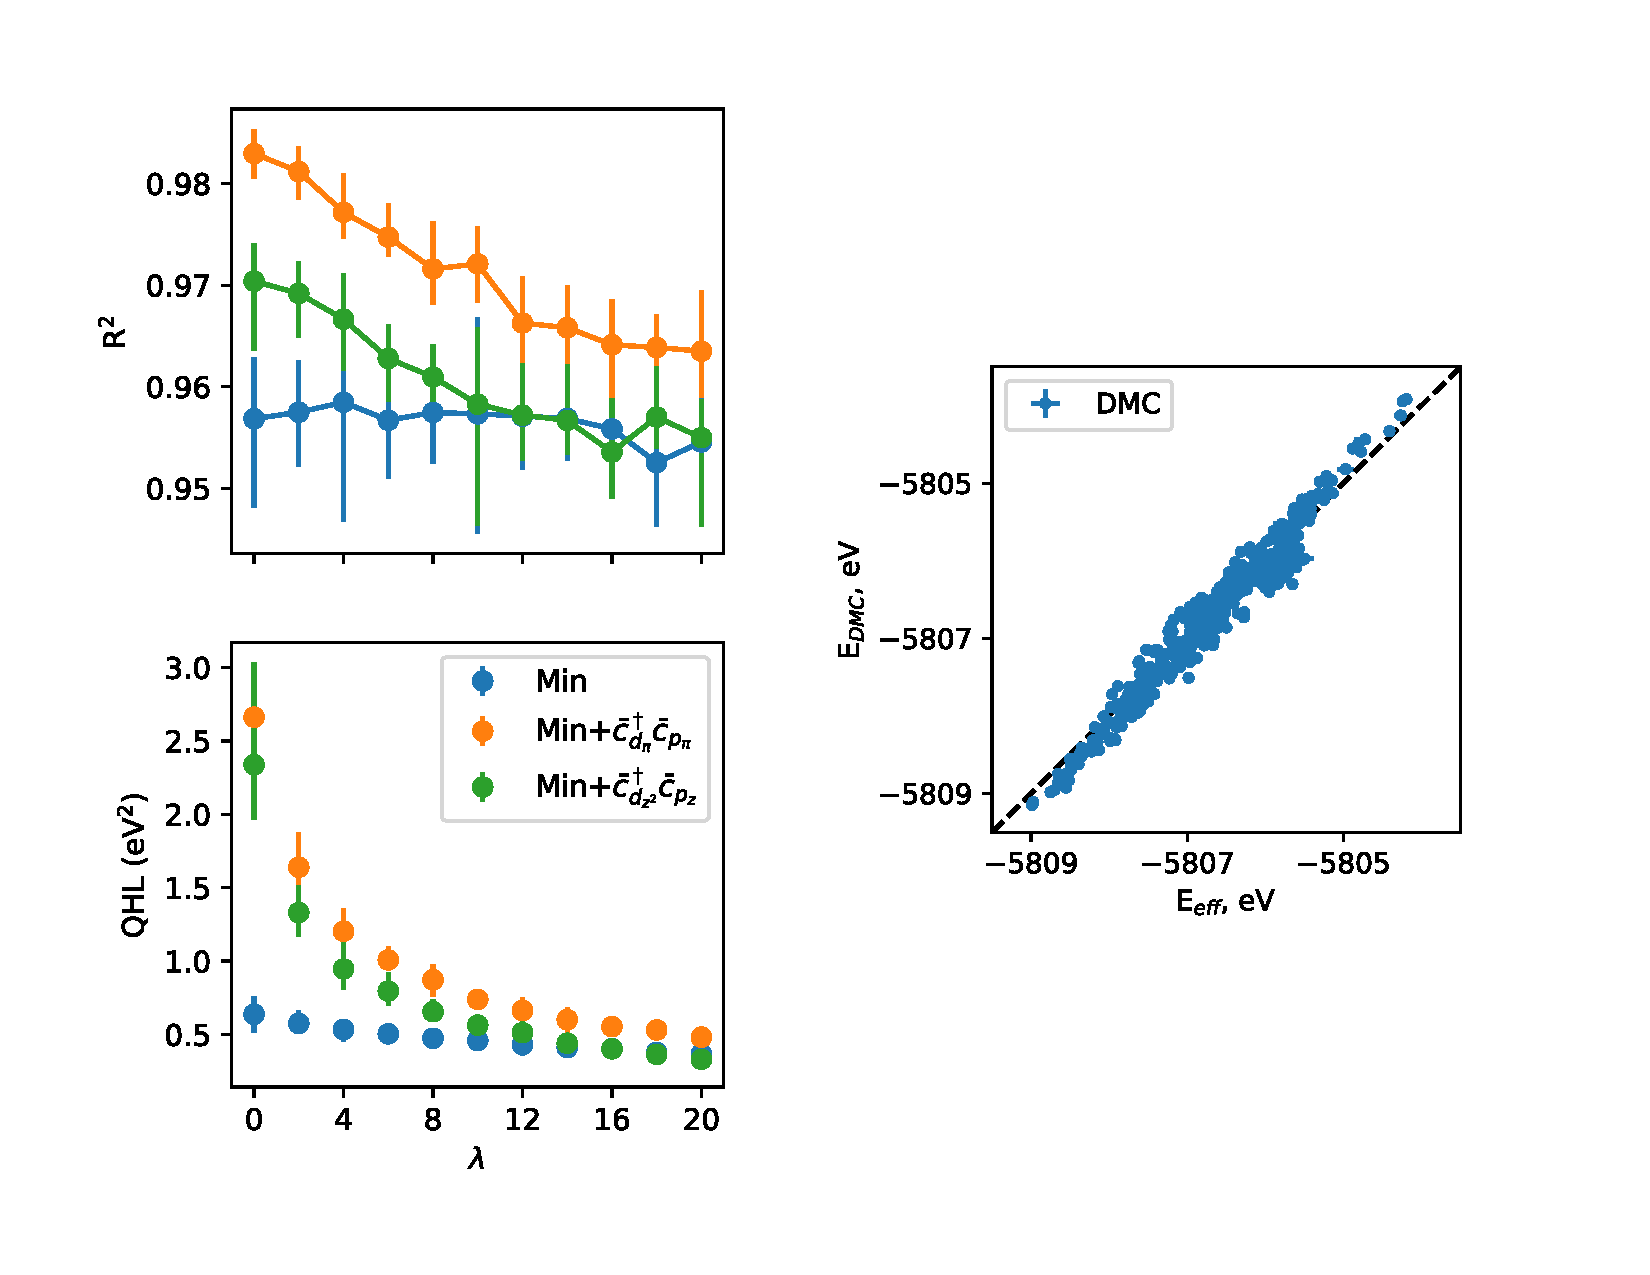
\includegraphics[width=0.7\linewidth]{../qwalk/old/ub3lyp_s1_/analysis/figs/prior_and_regr.pdf}
\caption{On the left, scores of the six candidate models at various $\lambda$ when fitting our effective theories using the cost function \eqref{eq:cost}. On the right we show predicted versus calculated energies for our low-energy sampled states for the minimal model fit at $\lambda = 20$.}
\label{fig:Prior}
\end{figure}

Figure \ref{fig:FinalED} presents the properties and eigenvalues of the lowest 30 eigenstates for three of the six fit models at $\lambda = 20$. 
In comparison one can view Figure \ref{fig:InitED} as the same figure for fits at $\lambda = 0$. 
At $\lambda = 20$ there are no outliers below 2eV in any of the three fit models. 
The ground states are similar for the three models, a feature also seen for the models fit at $\lambda = 0$.
Unlike at $\lambda = 0$, we see that the excited states of the three models are also very similar.
This pattern is also shared by the three other candidate models which are not shown. 
The additional constraint from asserting a prior has seemingly caused a single effective theory to emerge from our set of candidate models.
The values of the fit parameters for our six models can be seen in Table 1.
All the models share similar parameter values except the fifth model, Min$ + \bar{c}_{d_\pi}^\dagger \bar{c}_{p_\pi}, \bar{c}_{d_z^2}^\dagger \bar{c}_{4s}$, indicating that there are at least two different effective theories on $\mathcal{LE}$ which lead to identical low-energy eigenstates and spectra, describe the energies of our sample data accurately and satisfy our prior.
\textbf{Why does this happen?}

\begin{figure}[H]
\centering
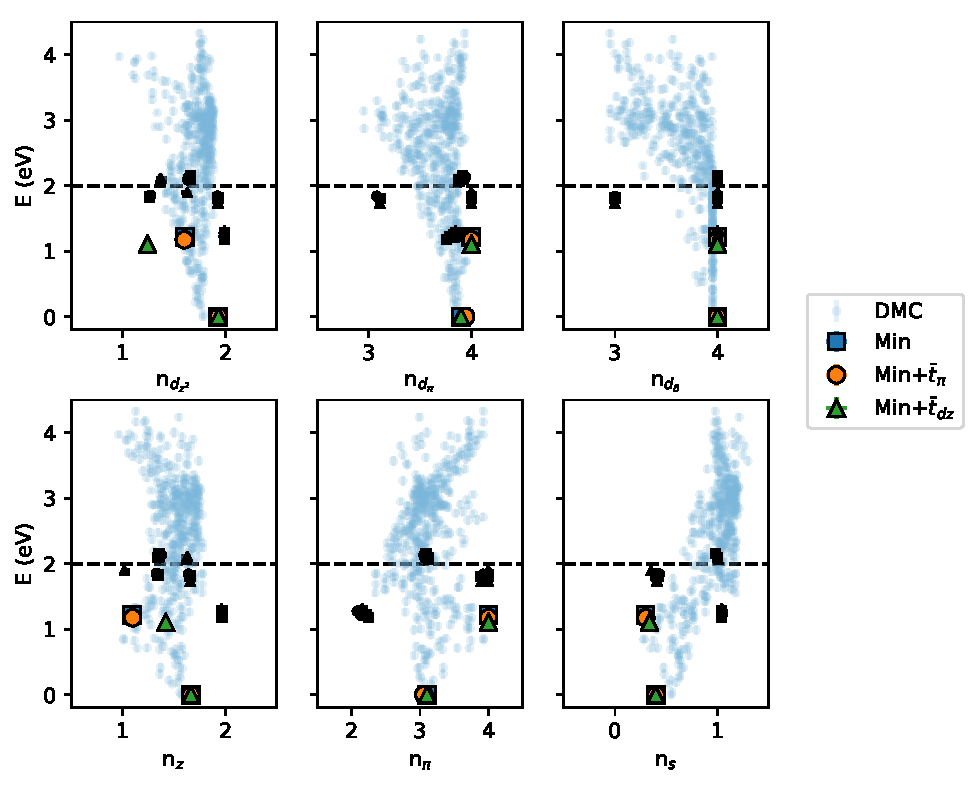
\includegraphics[width=0.7\linewidth]{../qwalk/old/ub3lyp_s1_/analysis/figs/final_ed.pdf}
\caption{Results of exact diagonalization showing the energies and properties of the first thirty eigenstates for three candidate models using linear regression with cost function \ref{eq:cost} and $\lambda = 20$. The ground state and first excited state are colored and have enlarged markers for clarity. Error bars are 95\% CI calculated by a bootstrap estimate.}
\label{fig:FinalED}
\end{figure}	
\begin{table}[H]
\begin{center}

\begin{tabular}{l|llllll}
&Min & Min & Min & Min & Min & Min \\
& & $ + \bar{c}_{d_\pi}^\dagger \bar{c}_{p_\pi}$ & $ + \bar{c}_{d_{z^2}}^\dagger \bar{c}_{p_z}$ & $ + \bar{c}_{d_\pi}^\dagger \bar{c}_{p_\pi}, \bar{c}_{4s}^\dagger \bar{c}_{p_z}$ & $ + \bar{c}_{d_\pi}^\dagger \bar{c}_{p_\pi}, \bar{c}_{d_z^2}^\dagger \bar{c}_{4s}$ & $ + \bar{c}_{d_z^2}^\dagger \bar{c}_{p_z}, \bar{c}_{d_z^2}^\dagger \bar{c}_{4s}$ \\ \hline 
$\epsilon_{d_{z^2}}$& 0.31(2)& 0.33(2)& 0.24(2)& 0.34(2)& 0.58(2)& 0.27(2)\\
$\epsilon_{d_\pi}$& 0.19(1)& 0.10(1)& 0.19(1)& 0.10(2)& 0.08(2)& 0.19(1)\\
$\epsilon_{d_\delta}$& 0.0(0)& 0.0(0)& 0.0(0)& 0.0(0)& 0.0(0)& 0.0(0)\\
$\epsilon_{4s}$& 2.16(4)& 2.24(6)& 2.22(3)& 2.23(6)& 1.2(2)& 2.2(6)\\
$\epsilon_{p_\pi}$& 1.7(4)& 1.84(4)& 1.72(2)& 1.83(4)& 2.13(4)& 1.71(4)\\
$\epsilon_{p_z}$& 0.93(5)& 0.98(5)& 1.06(3)& 0.96(6)& 1.73(7)& 0.99(7)\\
$t_\pi$& -0.57(1)& -0.45(2)& -0.58(1)& -0.46(3)& -0.47(2)& -0.57(1)\\
$t_{dz}$& 0.53(3)& 0.56(3)& 0.52(2)& 0.57(3)& 1.00(4)& 0.53(2)\\
$t_{sz}$& 0.88(3)& 0.89(1)& 0.84(2)& 0.87(3)& 1.26(6)& 0.8(3)\\
$t_{ds}$& 0.45(2)& 0.45(1)& 0.48(3)& 0.47(2)& 0.72(4)& 0.55(4)\\
$J_{sd}$& -0.6(1)& -0.9(1)& -0.7(1)& -0.9(1)& -0.4(1)& -0.7(1)\\
$U_s$& 4.0(1)& 3.6(3)& 3.9(1)& 3.6(2)& 4.5(2)& 3.9(1)\\
\end{tabular}
\\ $\ $
\\
Table 1: Parameters in eV for our six potential models when fit using \eqref{eq:cost} at $\lambda = 20$. 
\end{center}
\end{table}

\subsection{Comparisons to experiment and theory}
Our final regressed models accurately reproduce properties and energies of the lowest lying eigenstates as seen in modern APES experiments on the CuO molecule.
From Figure \ref{fig:FinalED} we see that the ground state of our effective theory has fully filled Cu 3d shell, nearly two electrons in O 2p$_z$ orbital, three in the O 2p$_\pi$ and around a quarter of an electron in the Cu 4s orbital.
An approximate electronic configuration for the ground state is therefore
be assigned 1$\sigma^2$1$\pi^4$1$\delta^4$2$\sigma^2$2$\pi^3$3$\sigma^0$ where the orbitals associated with the assignment are Cu 3d$_{z^2}$, Cu 3d$_\pi$, Cu 3d$_\delta$, O 2p$_z$, O 2p$_\pi$, and Cu 4s.
This state also has a total spin projection S$_z = \frac{1}{2}$.
This matches the well studied ground state electron configuration for the molecule $^2\Pi$.
There are two excited states around 1eV in energy, the first of which is a state with the following single excitation O 2p$_z \rightarrow$ O 2p$_\pi$, has the configuration 1$\sigma^2$1$\pi^4$1$\delta^4$2$\sigma^2$2$\pi^4$4$\sigma^0$, and S$_z = \frac{1}{2}$.
According to experiment there is also such a state at 1eV and is usually denoted as $^2X$.
A second excited state at 1.2 eV exists which corresponds to an excitation 
O 2p$_\pi \rightarrow$ Cu 4s, has configuration 1$\sigma^2$1$\pi^4$1$\delta^4$2$\sigma^2$2$\pi^2$4$\sigma^1$, and can either be S$_z = \frac{1}{2}, \frac{3}{2}$. 
This is also the lowest energy eigenstate which can be a spin quartet.
\textbf{ref} agree that this excitation should be the lowest spin quartet excitation, but argue that this state should be at an energy of 1.9 eV. 
Our model has a different spin quartet state with a full Cu d shell at 1.9 eV, corresponding to an excitation O 2p$_z \rightarrow$ Cu 4s, with configuration 1$\sigma^2$1$\pi^4$1$\delta^4$2$\sigma^1$2$\pi^4$4$\sigma^1$. 
There are another host of eigenstates for our models at 2 eV corresponding to singles excitations of the form Cu 3d $\rightarrow$ O 2p$_\pi$. 
This matches measurements which indicate that the lowest energy eigenstates with a single hole in the Cu 3d shell lie at 2.2 eV above the ground state.

Our model is more accurate than a single-particle model constructed using
density functional theory orbitals and eigenvalues. 
We consider a single-particle theory for the CuO molecule using restricted open-shell Kohn Sham (ROKS) eigenvalues and orbitals as single particle energies and states in our theory. 
This model is very inaccurate in describing the energy of any state with an occupied Cu 4s molecular orbital which it assigns to higher than 4 eV in energy above the ground state.
We believe this is due to this single particle method neglecting the heavy orbital relaxations between excited states, particularly in the $\sigma$ symmetry sector in which the Cu 4s orbital resides.

\section{Conclusions}
In this paper we systematically fit a many-body model for the neutral CuO molecule which can accurately reproduce the spectrum and properties of low-lying eigenstates seen in experiment using a \textit{ab-initio} QMC DMD method, and discuss the details of and developments in our model fitting procedure.
In particular, we study the problem of intruder states in our effective theories --- states which suffer from large extrapolations errors under our model ---  by connecting the existence of these states to our inability to access parts of $\mathcal{LE}$ when generating the low-energy wave function samples used to fit our models.
The intruder state issue is dealt by using our knowledge of $E_\text{ab}$ on the inaccessible parts of $\mathcal{LE}$ to construct a prior for our regression and enforcing it through an augmented ordinary linear regression cost function.
The resultant models fit using the augmented cost function do not contain any intruder states.
The fit models can accurately describe the energies and electron configurations of experimentally measured low-lying excitations with a much higher accuracy than effective single-particle theories generated by ROKS, particularly for quartet states.
We also discuss the non-uniqueness of effective theories by studying two different effective theories we built which produce almost identical spectra and eigenvectors and fit our sample data accurately.

We believe that the fitting procedure illustrated here can be used to generate effective theories for other strongly correlated systems and can be seen as a stepping stone towards developing a more robust downfolding methodology. 
A particularly interesting avenue may be developing effective theories for all neutral transition-metal oxide molecules (TMO), leading to a sequence of models across the transition metal atoms. 
From a methodology stand point, the work here indicates the need for a robust sampling method of $\mathcal{LE}$ which allows one to access the full space across different materials.
The existence of such a method would alleviate the need for the use of a prior to inject information about $E_\text{ab}$ on the inaccessible parts of $\mathcal{LE}$ and lead to a more conceptually and computationally direct model fitting procedure. 


\end{document}